\documentclass[14pt]{extarticle}
\usepackage{graphicx}
\usepackage[T1]{fontenc} 
\usepackage[margin=1in]{geometry}
\usepackage{hyperref}
\usepackage{amsmath}

% Custom captions: 1 pav.
\usepackage{caption}
\captionsetup[figure]{labelformat=empty}
\renewcommand{\thefigure}{\arabic{figure} pav.}

% Turinys vietoj Contents
\renewcommand{\contentsname}{Turinys}

\setlength{\textwidth}{7in}

\begin{document}

% Titulinis
\begin{titlepage}
	\begin{center}
		
\includegraphics[width=5cm]{images/ktu_logo.png}

		\textbf{Kauno technologijos universitetas}

		Informatikos fakultetas

		\vspace{3cm}

		\textbf{Komandinis darbas}

		\vspace{0.5cm}
		P176B101 Intelektikos pagrindai

	\end{center}

	\begin{flushright}

		\vfill

		\textbf{Arnas Bradauskas IFF-1/1}

		\textbf{Ignas Survila IFF-1/5}

		Studentai

		\vspace{0.2cm}

		\textbf{Arnas Nakrošis}

		Dėstytojas

	\end{flushright}

	\begin{center}
		Kaunas, 2024
	\end{center}

\end{titlepage}

% Turinys
\tableofcontents

\clearpage

\section{Duomenų rinkinys}

Duomenų rinkinyje egzistuoja tokie atributai:

\begin{itemize}
  \item work year - metai.
  \item experience level - darbuotojo patirties lygmuo.
  \item job title - darbo pozicijos pavadinimas.
  \item salary in usd - darbo atlyginimas JAV doleriais.
  \item company location - kompanijos lokacija.
  \item company size - kompanijos dydis.
\end{itemize}

\clearpage

\section{Metodų aprašymas}

Naudoti metodai: K-means ir SOM

\subsection{K-means}

Algoritmas suskirsto duomenis į K klasterių, kur kiekvienas taškas priklauso
klasteriui su artimiausiu vidurkiu. Algoritmas susidaro iš sių žingsnių:

\begin{enumerate}
  \item Inicializacija - atsitiktinai parenkame klasterių centrus.
  \item Priskytimas - Priskiriame kiekvieną duomenų tašką artimiausiam centrui priklausomai
    nuo Euklido atstumo.
  \item Atnaujinimas - apskaičiuojamas naujas kiekvieno klasterio centras
    pagal visų taškų vidurkį.
  \item Iteravimas - kartojame šiuos žingsnius kol pasiekiame konvergavimą 
    (centrai nebesikeičia ar keičiasi labai nežymiai).
\end{enumerate}

\subsection{SOM}

Dirbtinis neuroninis tinklas, naudojamas neprižiūrimam mokymui. Žingsniai:

\begin{enumerate}
  \item Inicializacija - atsitiktinai parenkame neuronų svorius.
  \item Apmokymas - Kiekvienam įvesties vektoriui randame BMU - neuroną, kuris
    turi artimiausią svorio vektorių. Atnaujiname BMU ir jo kaimyninius neuronus.
  \item Iteravimas - kartojame apmokymą daug iteracijų, po truputį mažindami
    mokymosi spartą ir kaiminystės dydį.
\end{enumerate}

\clearpage

\section{Atstumo metrika}

Algoritmų palyginimui naudojome Euklido atstumo metriką.
Turint du taškus \( \mathbf{p} = (p_1, p_2, \ldots, p_n) \) ir \( \mathbf{q} = (q_1, q_2, \ldots, q_n) \) n-dimencijų erdvėje, 
Euklido atstumas\( (\mathbf{p}, \mathbf{q}) \) tarp jų yra skaičiuojamas taip:

\[
d(\mathbf{p}, \mathbf{q}) = \sqrt{(p_1 - q_1)^2 + (p_2 - q_2)^2 + \cdots + (p_n - q_n)^2}
\]

\clearpage

\section{K-means}

Skaičiuojame silueto koeficientus ir inercijos reikšmes visoms įmanomoms atributų kombinacijoms, su klasterių kiekiu = [3,4,5].

\begin{figure}[!htbp]
	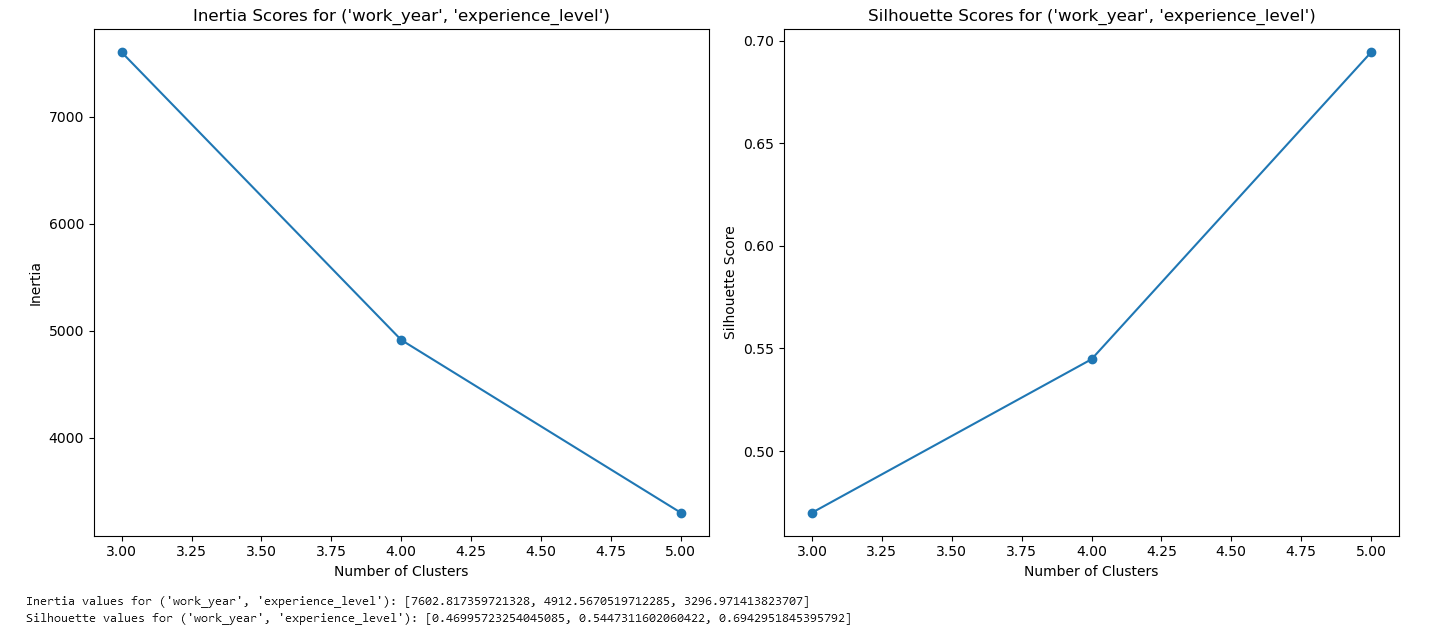
\includegraphics[width=\textwidth]{images/kmeans/1.png}
	\caption{\thefigure\ Grafikai "work year" x "experience level".}
\end{figure}

\begin{figure}[!htbp]
	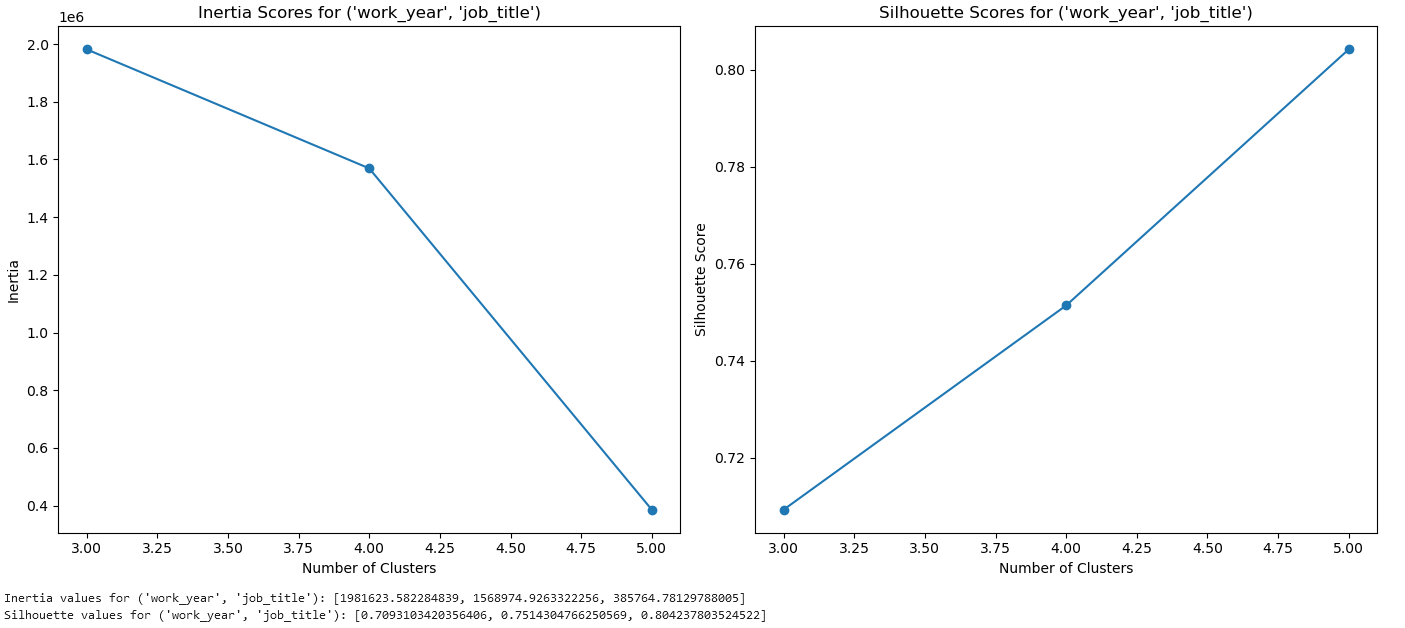
\includegraphics[width=\textwidth]{images/kmeans/2.png}
	\caption{\thefigure\ Grafikai "work year" x "job title".}
\end{figure}

\begin{figure}[!htbp]
	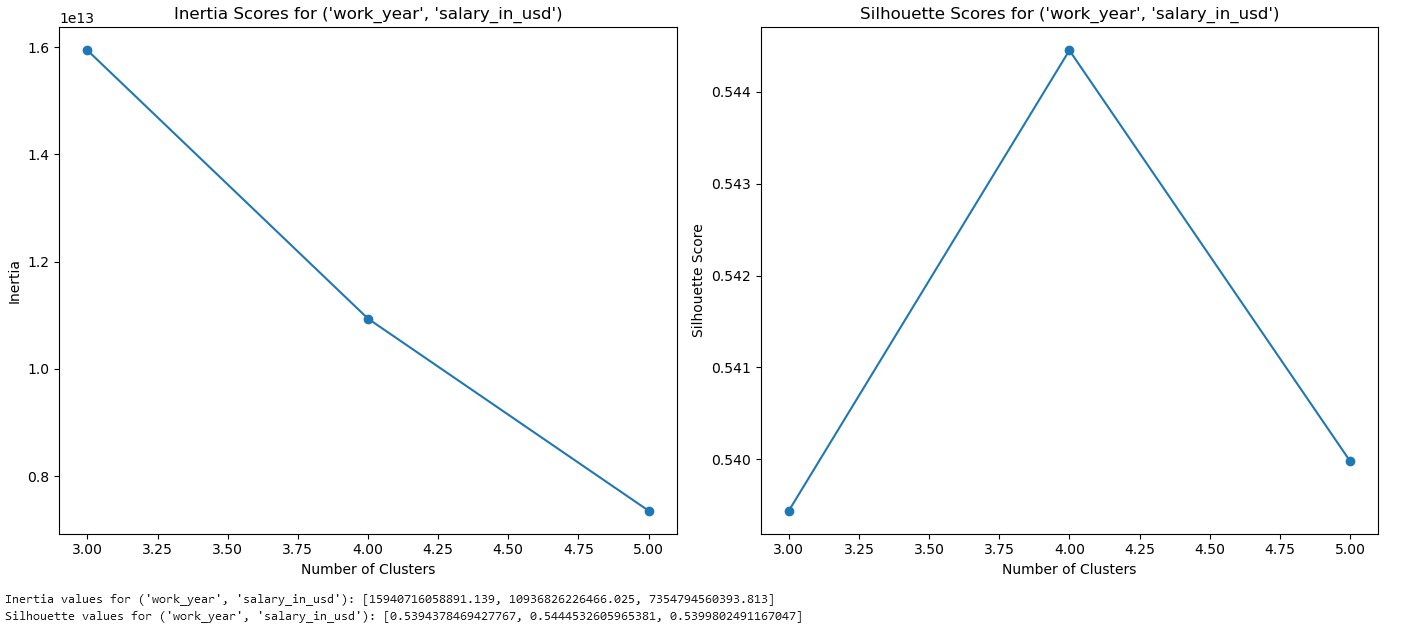
\includegraphics[width=\textwidth]{images/kmeans/3.png}
	\caption{\thefigure\ Grafikai "work year" x "salary in usd".}
\end{figure}

\begin{figure}[!htbp]
	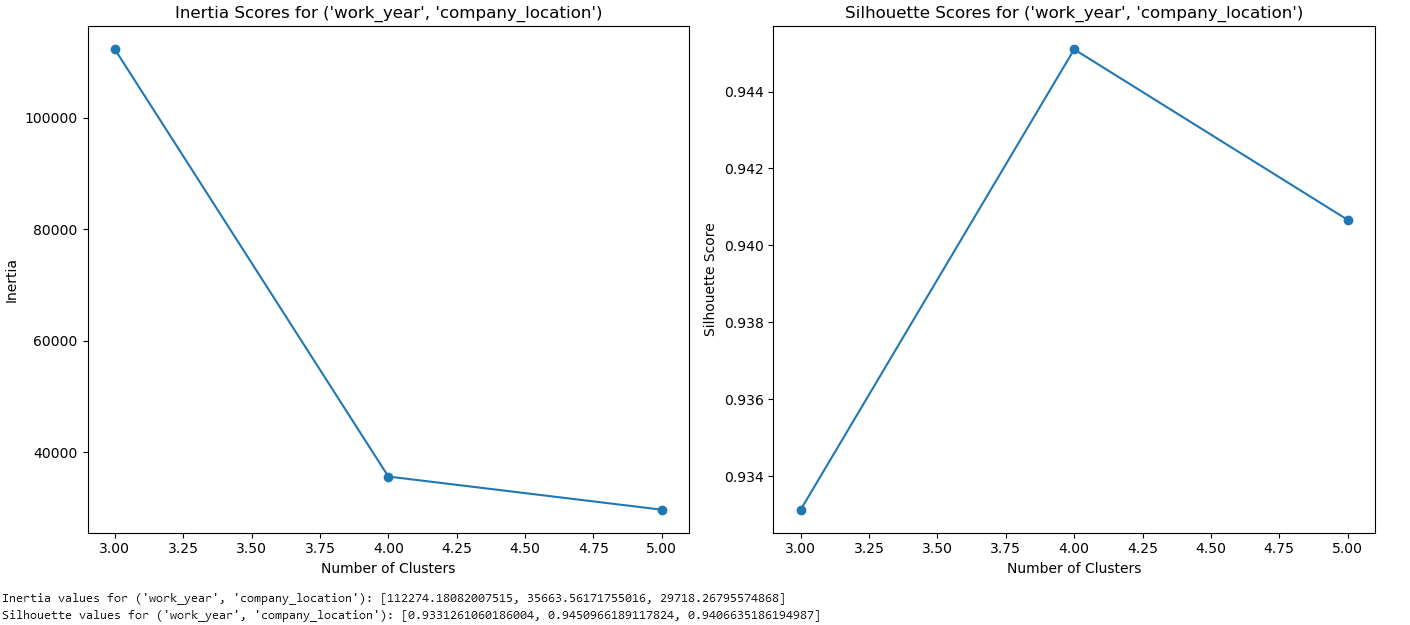
\includegraphics[width=\textwidth]{images/kmeans/4.png}
	\caption{\thefigure\ Grafikai "work year" x "company location".}
\end{figure}

\begin{figure}[!htbp]
	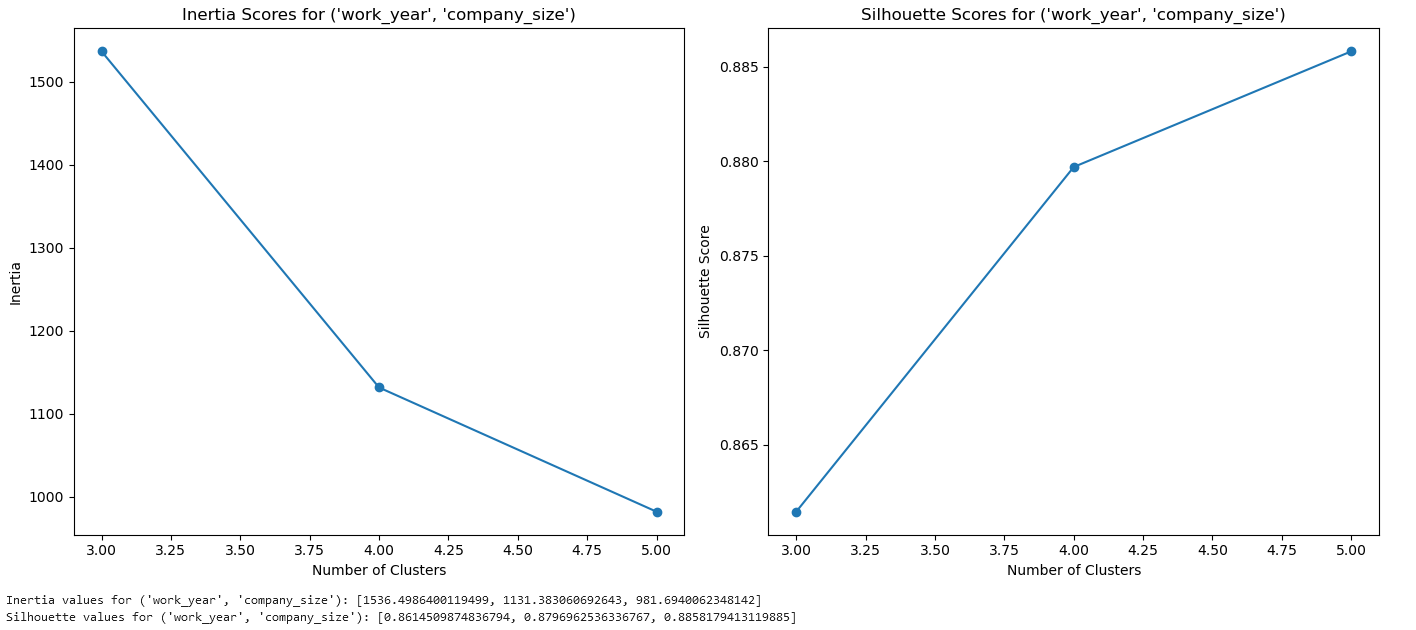
\includegraphics[width=\textwidth]{images/kmeans/5.png}
	\caption{\thefigure\ Grafikai "work year" x "company size".}
\end{figure}

\begin{figure}[!htbp]
	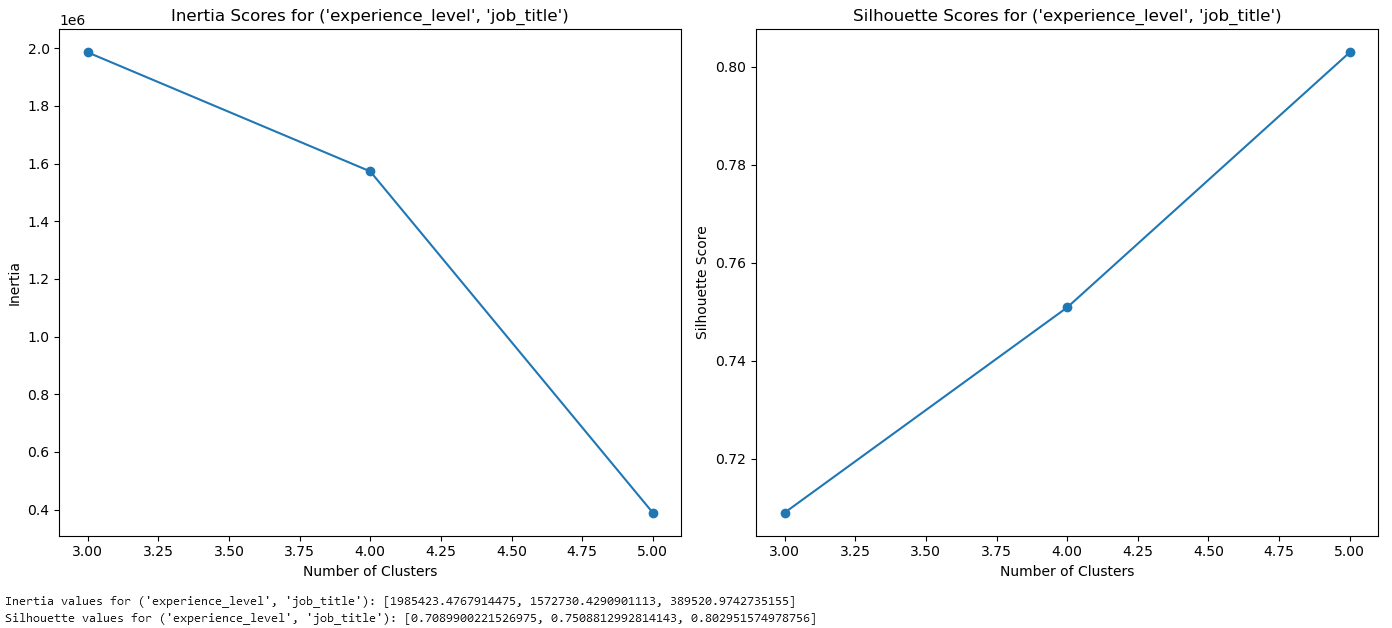
\includegraphics[width=\textwidth]{images/kmeans/6.png}
	\caption{\thefigure\ Grafikai "experience level" x "job title".}
\end{figure}

\begin{figure}[!htbp]
	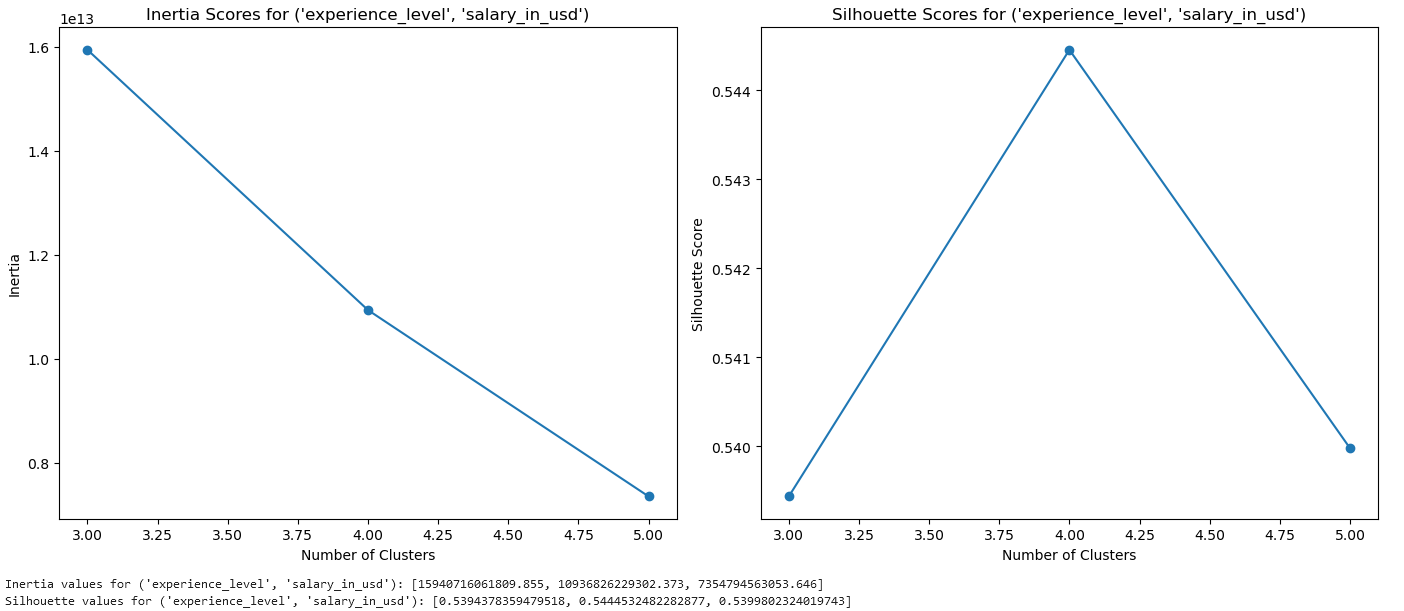
\includegraphics[width=\textwidth]{images/kmeans/7.png}
	\caption{\thefigure\ Grafikai "experience level" x "salary in usd".}
\end{figure}

\begin{figure}[!htbp]
	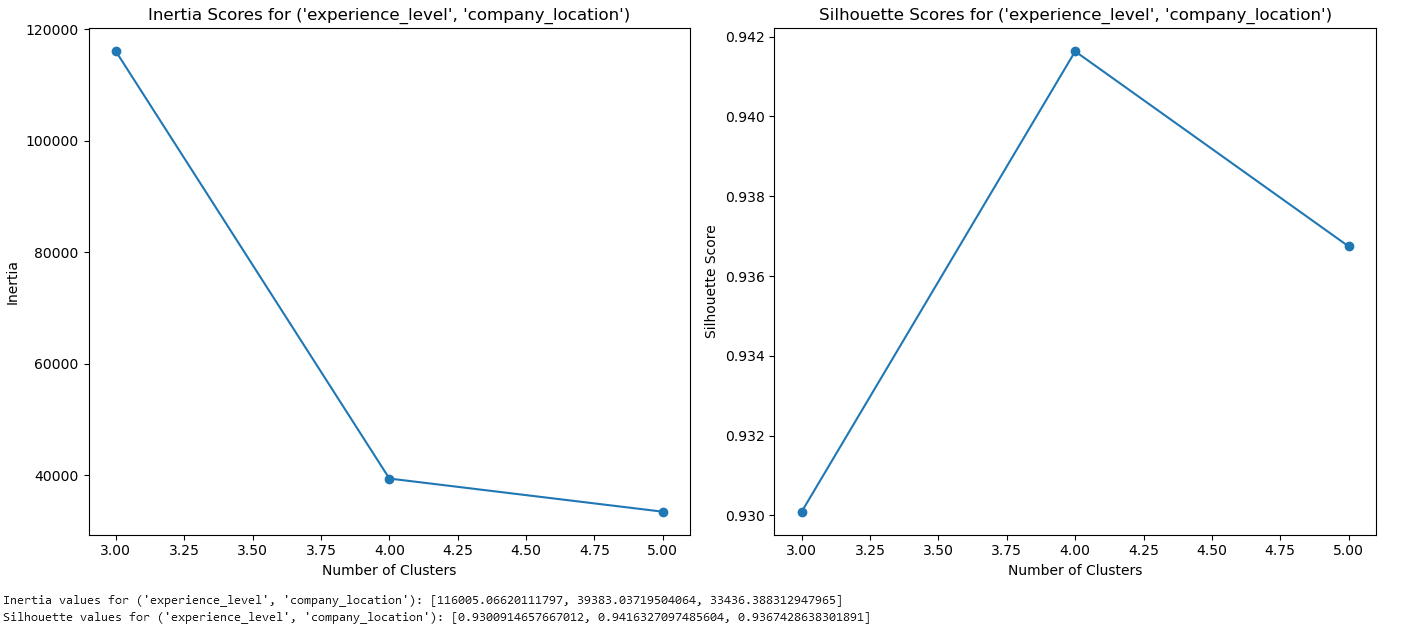
\includegraphics[width=\textwidth]{images/kmeans/8.png}
	\caption{\thefigure\ Grafikai "experience level" x "company location".}
\end{figure}

\begin{figure}[!htbp]
	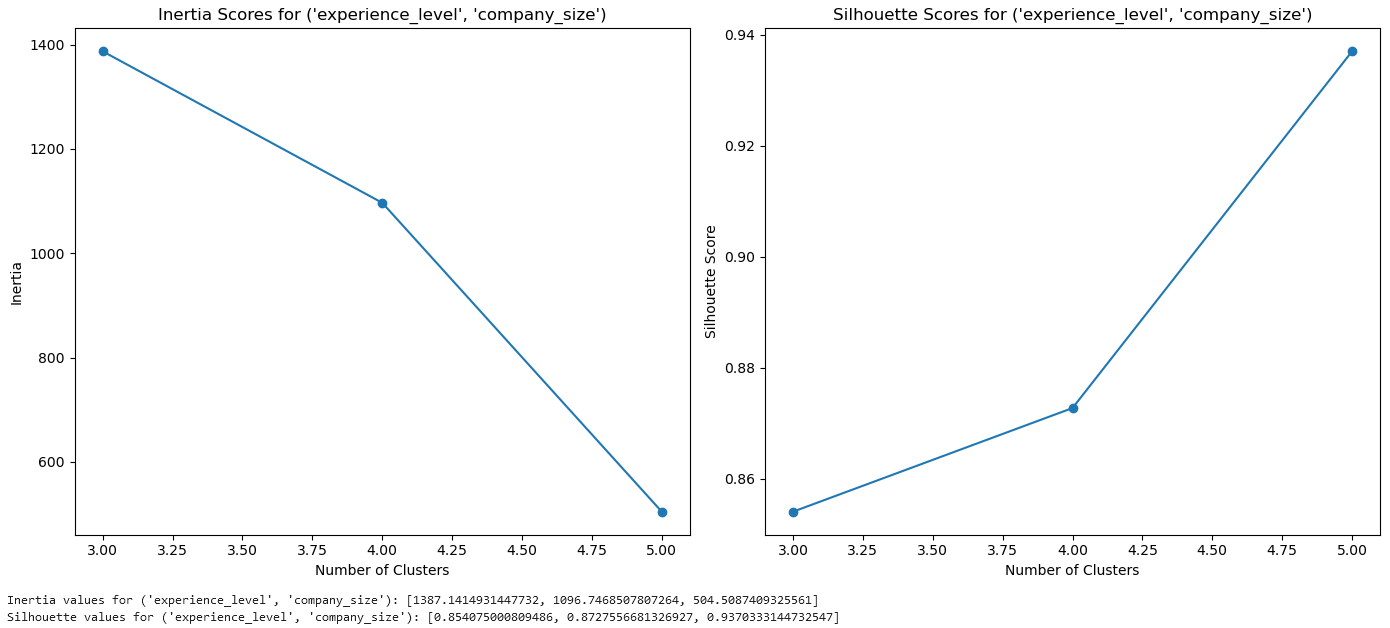
\includegraphics[width=\textwidth]{images/kmeans/9.png}
	\caption{\thefigure\ Grafikai "experience level" x "company size".}
\end{figure}

\begin{figure}[!htbp]
	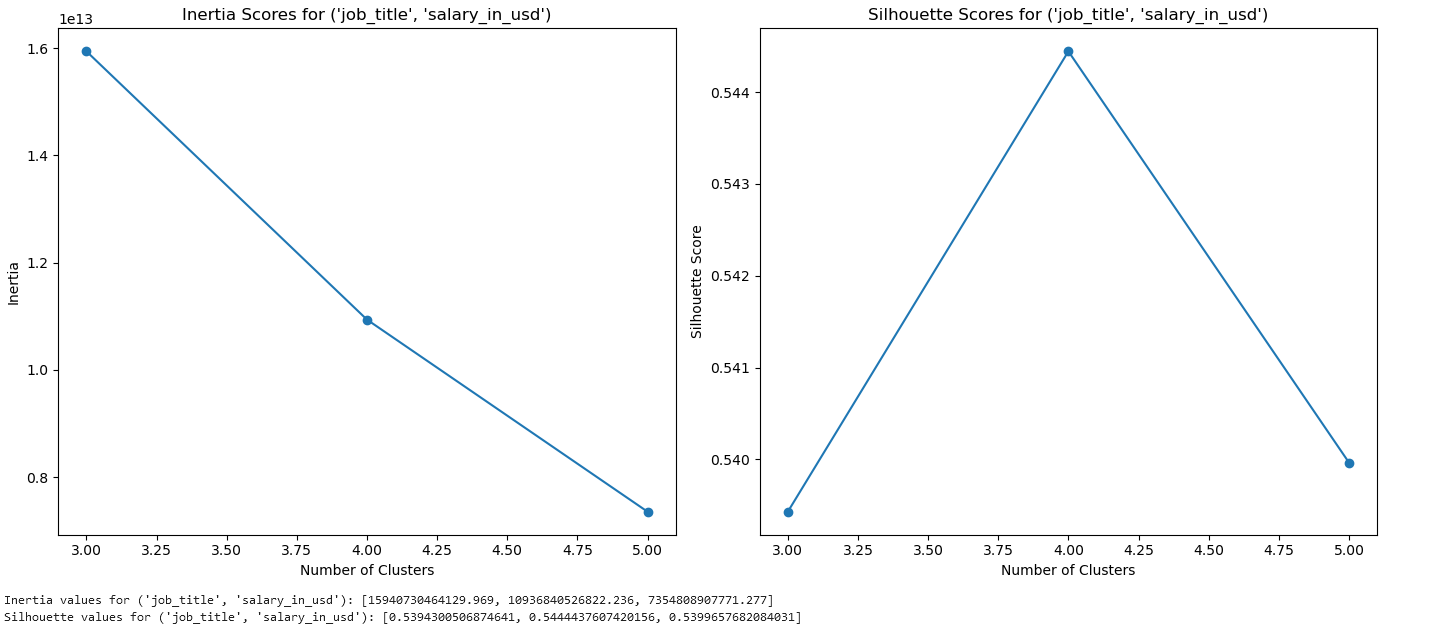
\includegraphics[width=\textwidth]{images/kmeans/10.png}
	\caption{\thefigure\ Grafikai "job title" x "salary in usd".}
\end{figure}

\begin{figure}[!htbp]
	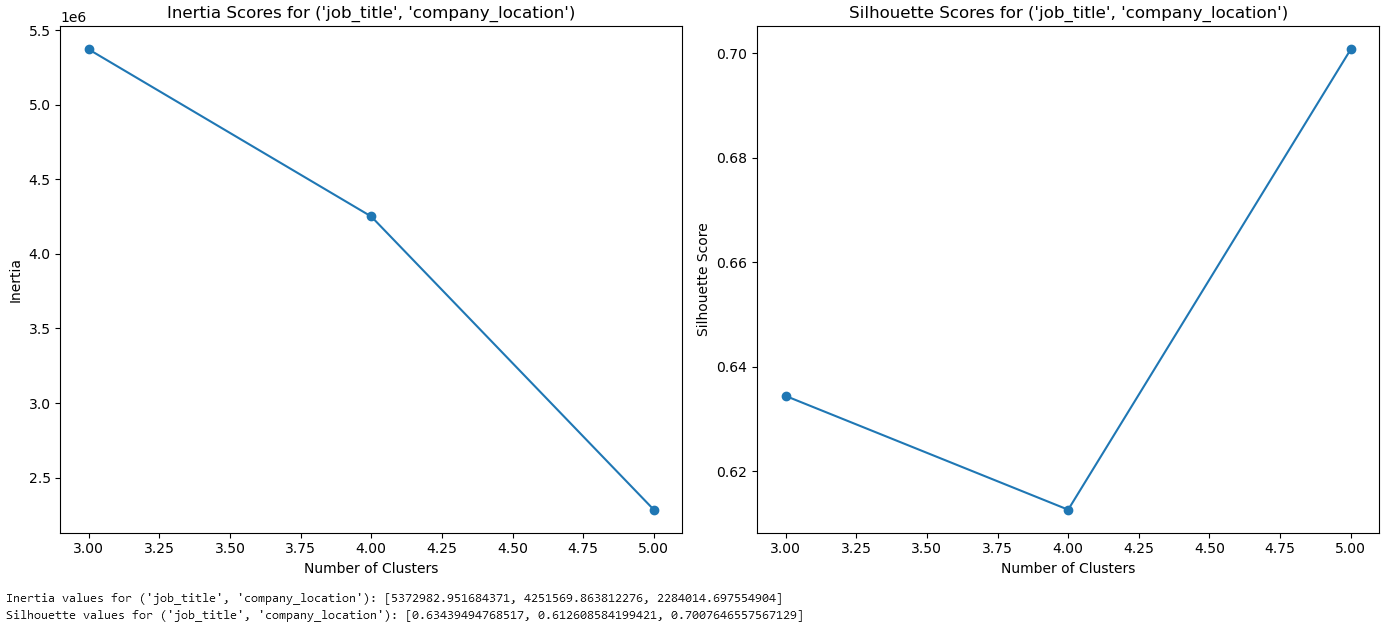
\includegraphics[width=\textwidth]{images/kmeans/11.png}
	\caption{\thefigure\ Grafikai "job title" x "company location".}
\end{figure}

\begin{figure}[!htbp]
	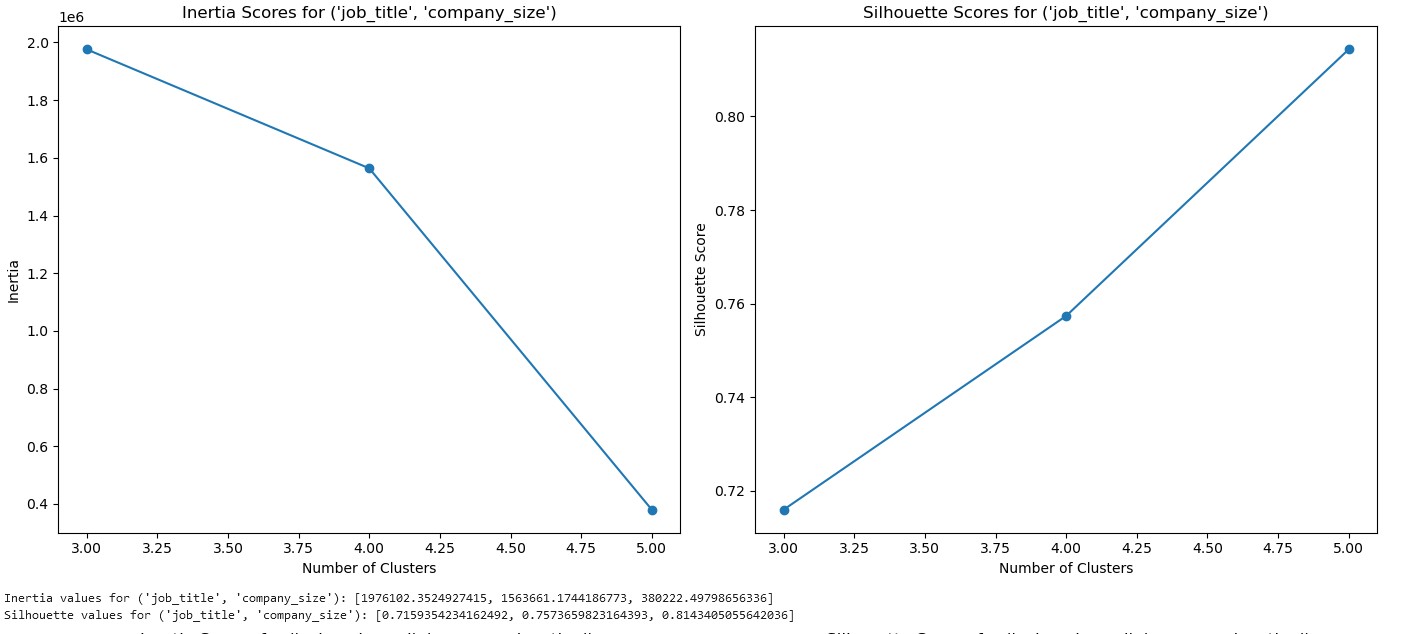
\includegraphics[width=\textwidth]{images/kmeans/12.png}
	\caption{\thefigure\ Grafikai "job title" x "company size".}
\end{figure}

\begin{figure}[!htbp]
	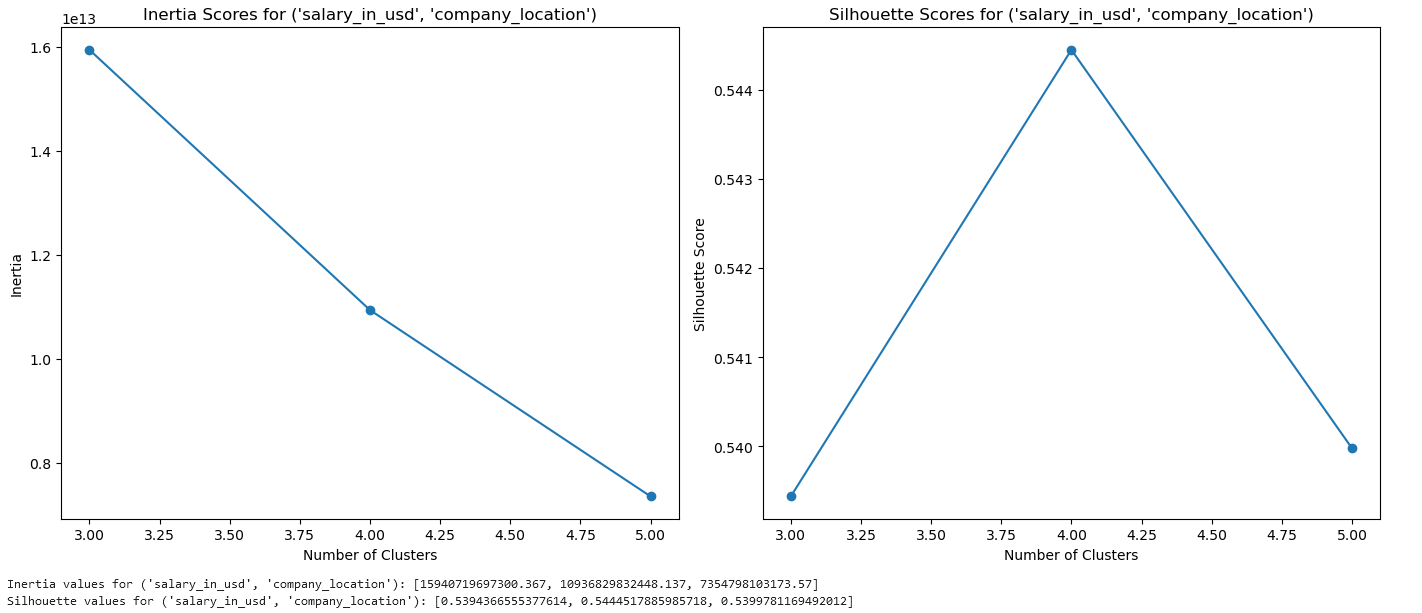
\includegraphics[width=\textwidth]{images/kmeans/13.png}
	\caption{\thefigure\ Grafikai "salary in usd" x "company location".}
\end{figure}

\begin{figure}[!htbp]
	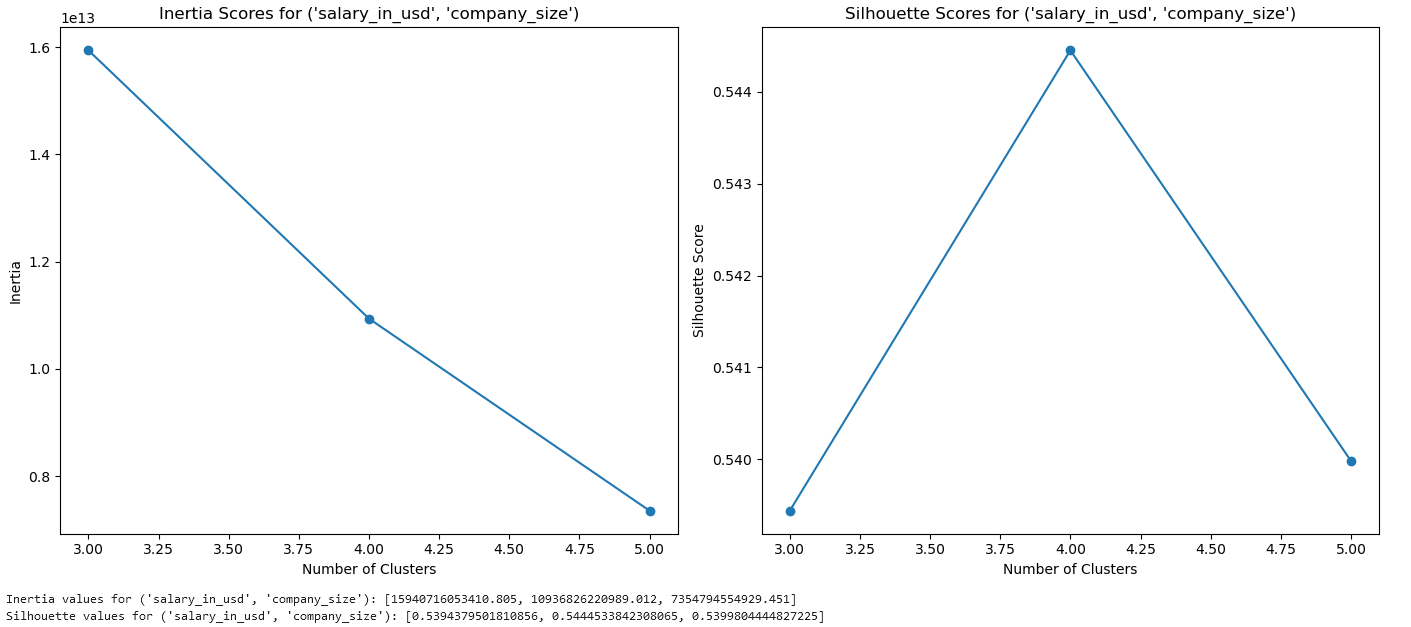
\includegraphics[width=\textwidth]{images/kmeans/14.png}
	\caption{\thefigure\ Grafikai "salary in usd" x "company size".}
\end{figure}

\begin{figure}[!htbp]
	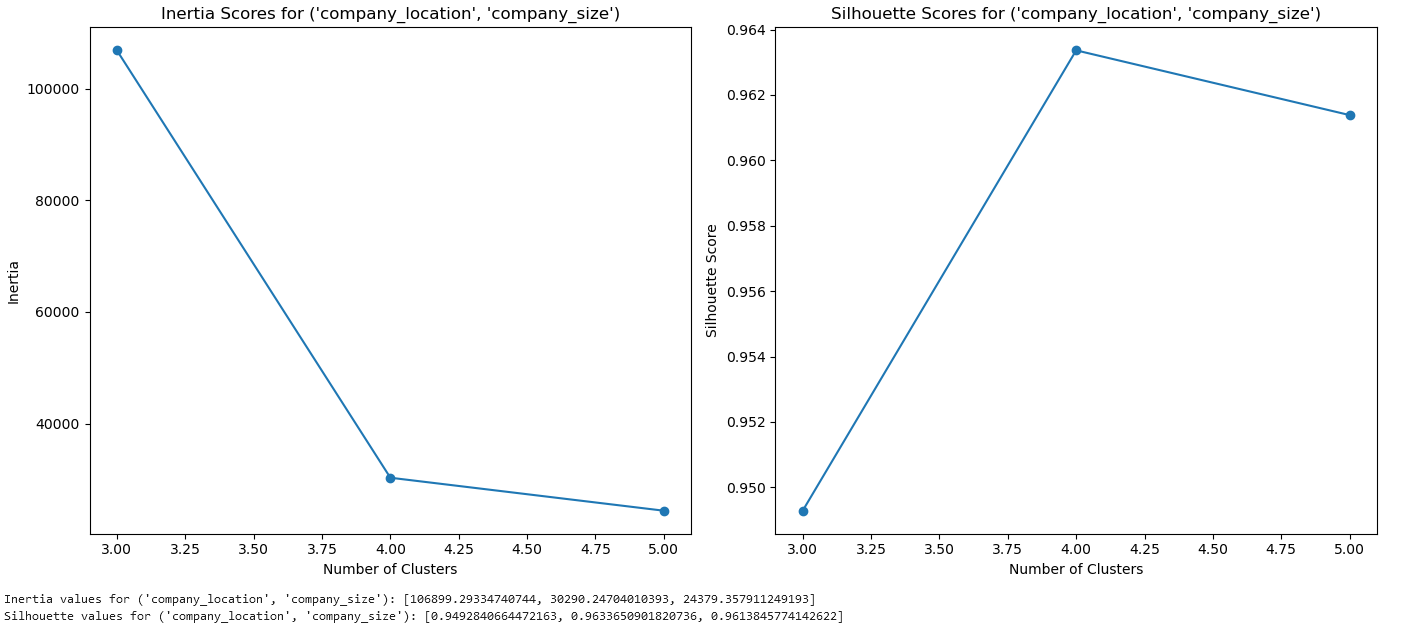
\includegraphics[width=\textwidth]{images/kmeans/15.png}
	\caption{\thefigure\ Grafikai "company location" x "company size".}
\end{figure}

Matome, jog geriausi rezultatai (didžiausias silueto koefocientas bei mažiausia inercija) gavosi su "experience level" x "company size" palyginimu,
todėl toliau jį naudosime kitiems skaičiavimams ir palyginimams.

\clearpage

\section{SOM}

Skaičiuojame silueto koeficientus "experience level" x "company size" su klasterių kiekiu = [3,4,5].

\begin{figure}[!htbp]
	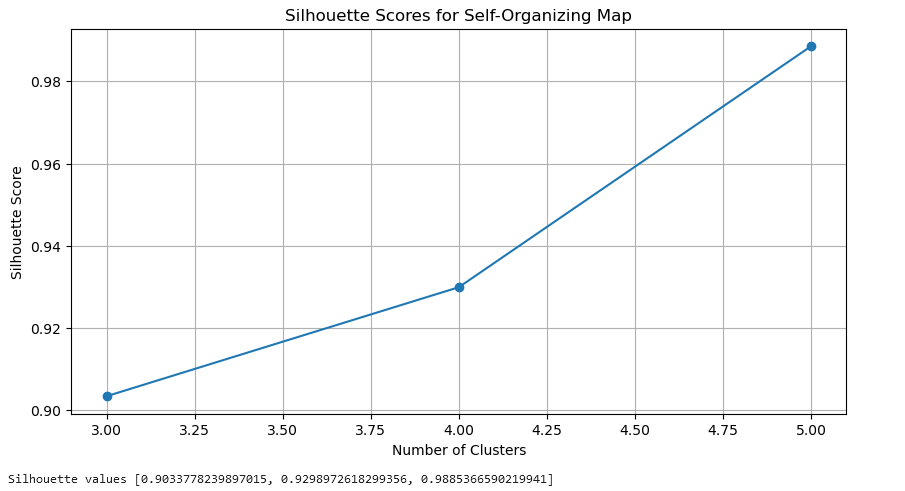
\includegraphics[width=\textwidth]{images/som/1.png}
	\caption{\thefigure\ SOM silueto grafikas "experience level" x "company size".}
\end{figure}

\clearpage

\section{K-means ir SOM palyginimas}

Galiausiai naudojame apskaičiuojame Euklido atstumą K-means ir SOM rezultatams, naudojame šiuos rezultatus kartu su siluetų koeficientais,
kad palyginti abu algoritmus.

\begin{figure}[!htbp]
	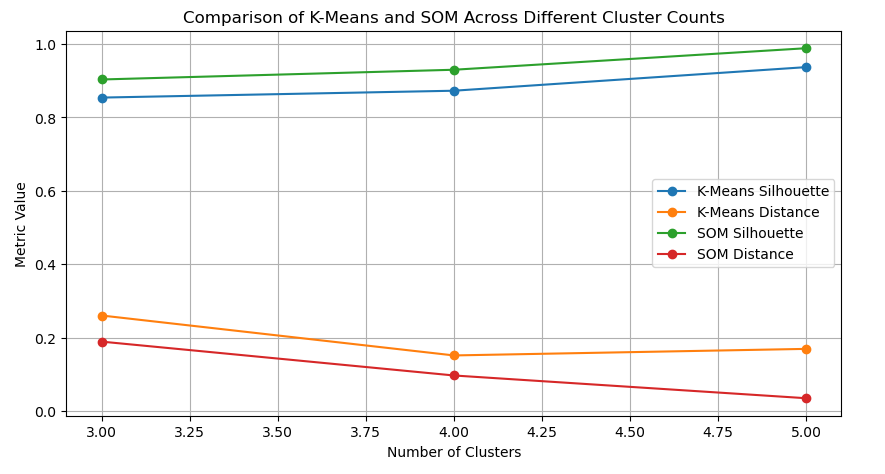
\includegraphics[width=\textwidth]{images/compare/1.png}
	\caption{\thefigure\ K-means ir SOM silueto koeficiento bei Euklido reikšmės palyginimas.}
\end{figure}

Matome, jog SOM algoritmas šiek tiek lenkia K-means lyginant ir siluetų koeficientus, ir Euklido atstumus. Tačiau abu algoritmai
tiekia sąlyginai gerus rezultatus.

\clearpage

\end{document}
